% Class 4 — Baseline & data check
\documentclass[
  english,
  aspectratio=169,
]{beamer}

\usepackage{babel}
\usepackage[utf8]{inputenc}
\usepackage[T1]{fontenc}
\usepackage{booktabs}
\usepackage{hyperref}
\usepackage{tikz}

\mode<beamer>{
  \definecolor{links}{HTML}{2A1B81}
  \hypersetup{colorlinks, linkcolor=, urlcolor=links}
  \usetheme{AGH}
}

% Keep title box below AGH header text
\makeatletter
\setbeamertemplate{title page}{%
  \vspace*{2.6cm}%
  \vbox{}%
  \vfill
  \hspace*{0.01\paperwidth}%
  \begingroup
  \centering
  \begin{beamercolorbox}[rounded=true,shadow=true,sep=8pt,wd=0.62\textwidth,center]{title}
    \usebeamerfont{title}\inserttitle\par
    \ifx\insertsubtitle\@empty\else
      \vskip0.25em
      {\usebeamerfont{subtitle}\usebeamercolor[fg]{subtitle}\insertsubtitle\par}%
    \fi
  \end{beamercolorbox}
  \vskip1em\par
  \begin{beamercolorbox}[sep=8pt,center]{author}
    \usebeamerfont{author}\insertauthor
  \end{beamercolorbox}
  \begin{beamercolorbox}[sep=8pt,center]{institute}
    \usebeamerfont{institute}\insertinstitute
  \end{beamercolorbox}
  \endgroup
  \vfill
}
\makeatother

\title[When Do GNNs Help?]{When Do Graph Neural Networks Help?}
\subtitle{Class 4 --- Baseline and Data Check}
\author[M.~Bro\'{s} \& M.~Burda]{%
  Micha\l{} Bro\'{s}\inst{1}
  \and
  Micha\l{} Burda\inst{1}
}
\institute[AGH]{%
  \inst{1}%
  Computational Intelligence \\
  Prof.~Adrian Horzyk \\
  AGH University of Krakow
}
\date{}

\begin{document}

\begin{frame}[plain]
  \titlepage
\end{frame}

%#####################################################################
\section{Reminder}
%#####################################################################

\begin{frame}{01~~Project reminder}
  \begin{block}{Research question}
    When do GNNs beat MLP / XGBoost, and how much edge noise
    can they survive before losing?
  \end{block}

  \begin{itemize}
    \item \textbf{H1:} on clean similar graphs GNNs win;
      after enough fake edges, tabular models catch up.
    \item \textbf{H2:} on mixed graphs, tabular models may win from the start.
  \end{itemize}

  \vspace{0.5em}
  \textbf{Class 4 focus:} working baseline + data audit + first reproducible
  evaluation on a \emph{clean} graph (no edge corruption yet).
\end{frame}

%#####################################################################
\section{Data audit}
%#####################################################################

\begin{frame}{02~~Data audit --- Cora}
  \begin{block}{Planetoid Cora (PyTorch Geometric)}
    \scriptsize
    \renewcommand{\arraystretch}{1.15}
    \begin{tabular}{ll}
      Nodes & 2708 \\
      Undirected edges & 5278 \\
      Features & 1433 (row-normalised bag-of-words) \\
      Classes & 7 \\
      Train / val / test & 140 / 500 / 1000 \\
      Split overlap & \textbf{0} (no leakage between masks) \\
    \end{tabular}
  \end{block}

  \vspace{0.4em}
  {\small Features scaled to $[0,1]$; class sizes uneven (largest class $\approx$ 818 nodes).}
\end{frame}

\begin{frame}{03~~Why this audit matters}
  \begin{itemize}
    \item Same fixed masks for \textbf{every} model (fair comparison)
    \item Preprocessing / normalisation does not peek at test labels
    \item Overlap check = 0 $\Rightarrow$ no train--test leakage in splits
    \item Small, fast dataset $\Rightarrow$ easy multi-seed runs on a laptop
  \end{itemize}

  \vspace{0.6em}
  \begin{alertblock}{Scope for today}
    Clean Cora only. Edge deletion / fake edges and mixed graphs come next.
  \end{alertblock}
\end{frame}

%#####################################################################
\section{Baseline protocol}
%#####################################################################

\begin{frame}{04~~Models compared}
  \begin{columns}[T]
    \begin{column}{0.48\textwidth}
      \begin{block}{No graph}
        \begin{itemize}
          \item MLP (2-layer)
          \item XGBoost on node features
        \end{itemize}
      \end{block}
    \end{column}
    \begin{column}{0.48\textwidth}
      \begin{block}{With graph}
        \begin{itemize}
          \item GCN (2-layer)
        \end{itemize}
      \end{block}
    \end{column}
  \end{columns}

  \vspace{0.7em}
  \textbf{Fair protocol}
  \begin{itemize}
    \item Identical Planetoid train/val/test masks
    \item 5 seeds: 0--4; report mean $\pm$ std
    \item MLP/GCN: 200 epochs, Adam, early pick by best val accuracy
    \item Code: \texttt{code/scripts/run\_baselines.py}
  \end{itemize}
\end{frame}

%#####################################################################
\section{Results}
%#####################################################################

\begin{frame}{05~~First results --- Cora test accuracy}
  \begin{block}{Mean $\pm$ std over 5 seeds}
    \renewcommand{\arraystretch}{1.25}
    \begin{tabular}{lcc}
      \textbf{Model} & \textbf{Test accuracy} & \textbf{Test macro-F1} \\
      \hline
      XGBoost & $0.527 \pm 0.006$ & $0.514 \pm 0.006$ \\
      MLP & $0.591 \pm 0.008$ & $0.572 \pm 0.008$ \\
      GCN & $\mathbf{0.818 \pm 0.005}$ & $\mathbf{0.806 \pm 0.005}$ \\
    \end{tabular}
  \end{block}

  \vspace{0.5em}
  Saved under \texttt{RESULTS/baseline\_cora\_*.csv} and \texttt{data\_audit.json}.
\end{frame}

\begin{frame}{06~~Clean-graph takeaway}
  \begin{itemize}
    \item On clean Cora, \textbf{GCN clearly beats} feature-only baselines
      ($\approx +23$ pp vs MLP, $+29$ pp vs XGBoost).
    \item Supports the starting point of \textbf{H1}: with good (similar)
      connections, the graph helps.
  \end{itemize}

  \vspace{0.4em}
  \begin{center}
  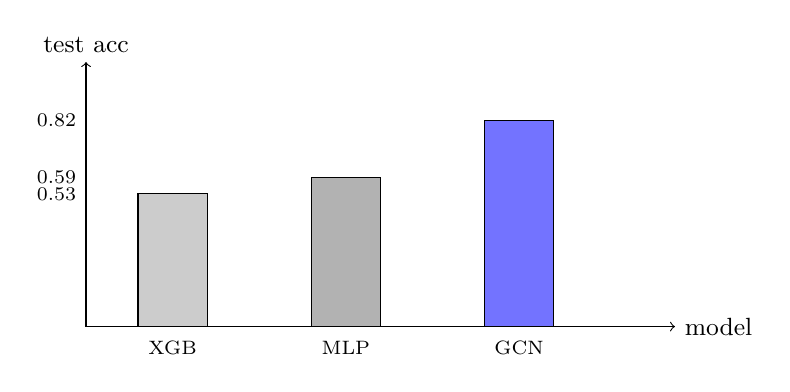
\begin{tikzpicture}[x=2.2cm,y=3.2cm]
    \draw[->] (0,0) -- (3.4,0) node[right] {\small model};
    \draw[->] (0,0) -- (0,1.05) node[above] {\small test acc};
    \draw[fill=gray!40] (0.3,0) rectangle (0.7,0.527);
    \draw[fill=gray!60] (1.3,0) rectangle (1.7,0.591);
    \draw[fill=blue!55] (2.3,0) rectangle (2.7,0.818);
    \node[below] at (0.5,-0.02) {\scriptsize XGB};
    \node[below] at (1.5,-0.02) {\scriptsize MLP};
    \node[below] at (2.5,-0.02) {\scriptsize GCN};
    \node[left] at (0,0.527) {\scriptsize 0.53};
    \node[left] at (0,0.591) {\scriptsize 0.59};
    \node[left] at (0,0.818) {\scriptsize 0.82};
  \end{tikzpicture}
  \end{center}
\end{frame}

%#####################################################################
\section{Experiment A}
%#####################################################################

\begin{frame}{07~~Experiment A --- delete real edges}
  \textbf{Idea:} randomly remove undirected edges:
  $0\%, 20\%, 40\%, 60\%, 80\%, 100\%$.

  \begin{itemize}
    \item Same Cora splits, 5 seeds, models: MLP / XGBoost / GCN
    \item Tabular models should stay flat (they ignore edges)
    \item GCN should fall as structure disappears
  \end{itemize}
\end{frame}

\begin{frame}{08~~Experiment A results (Cora)}
  \begin{block}{Test accuracy (mean over 5 seeds)}
    \scriptsize
    \renewcommand{\arraystretch}{1.15}
    \begin{tabular}{lcccccc}
      \textbf{Model} & 0\% & 20\% & 40\% & 60\% & 80\% & 100\% \\
      \hline
      XGBoost & 0.527 & 0.527 & 0.527 & 0.527 & 0.527 & 0.527 \\
      MLP & 0.593 & 0.592 & 0.592 & 0.592 & 0.592 & 0.592 \\
      GCN & \textbf{0.818} & 0.793 & 0.764 & 0.726 & 0.673 & 0.594 \\
    \end{tabular}
  \end{block}

  \vspace{0.45em}
  {\small Saved in \texttt{RESULTS/expA\_cora\_summary.csv}.}
\end{frame}

\begin{frame}{09~~Experiment A --- conclusions}
  \begin{itemize}
    \item MLP / XGBoost are \textbf{flat} (as expected).
    \item GCN drops smoothly: $0.82 \rightarrow 0.79$ (20\%)
      $\rightarrow 0.76$ (40\%) $\rightarrow 0.73$ (60\%)
      $\rightarrow 0.67$ (80\%) $\rightarrow 0.59$ (100\%).
    \item Even after \textbf{removing 80\%} of edges, GCN still beats MLP
      ($0.67 > 0.59$).
    \item At \textbf{100\%} deletion, GCN $\approx$ MLP ($0.594$ vs $0.592$).
    \item Near 30\%: between 20\% and 40\% --- GCN still clearly ahead
      ($\approx 0.79$--$0.76$).
  \end{itemize}

  \vspace{0.35em}
  \begin{block}{Takeaway}
    On Cora, a lot of graph structure can be removed before GCN loses its
    advantage. Next: fake edges (Experiment B).
  \end{block}
\end{frame}

\begin{frame}{10~~Next steps}
  \begin{enumerate}
    \item \textbf{Experiment B:} add fake edges $0\% \rightarrow 75\%$
      (hypothesised breaking point $\sim$30\%)
    \item Add a \textbf{mixed} dataset (Roman-empire / filtered Chameleon)
    \item Extend models: GraphSAGE, GAT
  \end{enumerate}

  \vspace{0.5em}
  \begin{block}{Class 4 takeaway}
    Baseline + data audit + Experiment A are done.
    Graph helps on clean Cora; advantage shrinks as edges are deleted,
    but survives until nearly all edges are gone.
  \end{block}
\end{frame}

\end{document}
